\documentclass{article}
\usepackage[T1]{fontenc}
\usepackage{lmodern}
\usepackage{graphicx}
\usepackage{amsmath,amssymb}
\usepackage[a4paper,margin=2cm]{geometry}
\usepackage[absolute,overlay]{textpos}
\setlength{\TPHorizModule}{1mm}
\setlength{\TPVertModule}{1mm}
\usepackage[indonesian]{babel}
\usepackage{hyperref}
\setlength{\emergencystretch}{2em}
% unit: Halaman 15

\begin{document}

% === Halaman 15 (python/native) ===

(b) P + (-P) = O, di sini O adalah titik di infinity 

15

P’= -P adalah elemen invers:

   P + P’ = P + (-P) = O 

O adalah elemen netral:

   P + O = O + P = P

Sumber gambar: Andreas Steffen, Elliptic Curve Cryptography

% deskripsi: gambar native xref 81
\noindent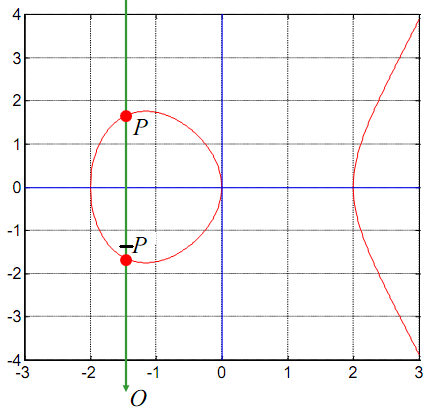
\includegraphics[width=0.85\textwidth]{../../images/python/page_015_img_01.png}

\end{document}
